\documentclass[11pt]{article}
\usepackage{latexsym}
\usepackage{amsmath}
\usepackage{amssymb}
\usepackage{amsthm}
\usepackage{epsfig}
\usepackage{psfig}
\usepackage{color}

\newcommand{\handout}[5]{
  \noindent
  \begin{center}
  \framebox{
    \vbox{
      \hbox to 5.78in { {\bf 6.851: Advanced Data Structures } \hfill #2 }
      \vspace{4mm}
      \hbox to 5.78in { {\Large \hfill #5  \hfill} }
      \vspace{2mm}
      \hbox to 5.78in { {\em #3 \hfill #4} }
    }
  }
  \end{center}
  \vspace*{4mm}
}

\newcommand{\lecture}[4]{\handout{#1}{#2}{#3}{Scribe: #4}{Lecture #1}}

\newtheorem{theorem}{Theorem}
\newtheorem{corollary}[theorem]{Corollary}
\newtheorem{lemma}[theorem]{Lemma}
\newtheorem{observation}[theorem]{Observation}
\newtheorem{proposition}[theorem]{Proposition}
\newtheorem{definition}[theorem]{Definition}
\newtheorem{claim}[theorem]{Claim}
\newtheorem{fact}[theorem]{Fact}
\newtheorem{assumption}[theorem]{Assumption}

% 1-inch margins, from fullpage.sty by H.Partl, Version 2, Dec. 15, 1988.
\topmargin 0pt
\advance \topmargin by -\headheight
\advance \topmargin by -\headsep
\textheight 8.9in
\oddsidemargin 0pt
\evensidemargin \oddsidemargin
\marginparwidth 0.5in
\textwidth 6.5in

\parindent 0in
\parskip 1.5ex
%\renewcommand{\baselinestretch}{1.25}

\begin{document}

\lecture{2 --- 02/09, 2012}{Spring 2012}{Prof.\ Erik Demaine}{Erek Speed, Victor Jakubiuk}

\section{Overview}

The main idea of the persistent data structures is that when you make a change in the past, you get an entirely new universe. A more science-fiction approach to time travel is that you can make changes in the past and see its result not only in the current state of the data structure, but also all the changes in between the past and now.

We maintain one timeline of updates and queries for a persistent data structure:

[img of a timeline]

blah blah blah

Normally, we always append the operations to the end of the timeline (present time). With retroactive data structures we can do that in the past too.

\section{Retroactivity}

The following operations are supported by retroactive DS:

\begin{itemize}
\item {\em Insert(t, update)} - inserts operation ``update'' at time $t$
\item {\em Delete(t)} - deletes the operation at time $t$
\item {\em Query(t, query)} queries the DS with a ``query'' at time $t$
\end{itemize}

Uppercase Insert indicates an operation on retroactive DS, lowercase is the operation on the actual DS.

You can think of time $t$ as integers, but a better approach is to use an order-maintanance DS to avoid using non-integers (in case you want to insert an operation between $t$ and $t+1$), as mentioned in the first lecture.

There are three types of retroactivity:
\begin{itemize}
\item {\em Partial} - Query always done at $t = \infty$ (now)
\item {\em Full} - Query at any time $t$ (possibly in the past)
\item {\em Nonoblivious} - 
\end{itemize}

\subsubsection{Priority Queues}
Now, let us move onto some more positive results.  Priority queues represent a DS where retroactive operations potentially create chain reactions but we have still obtained some nice results for.  The main operations are $insert$ and $delete$-$min$ which we would like to retroactively $Insert$ and $Delete$.

\begin{claim}
	It is possible to implement a partially retroactive priority queue with only $O(\lg n)$ overhead per partially retroactive operation.
\end{claim}

Because of the presence of $delete$-$min$, the set of operations on priority queues is non-commutative.  The order of updates now clearly matters, and $Insert$ing a $delete$-$min$ retroactively has the potential to cause a chain reaction which changes everything that comes afterward. \\

To develop an intuition for how our DS changes given a retroactive operation, it is helpful to plot it on a two dimensional plane.  The $x$-axis represents time and $y$-axis represents key value. Every $insert(t,k)$ operation creates a horizontal ray that starts at point $(t,k)$ and shoots to the right (See Fig. \ref{fig-pqinsert}).

\begin{figure}[ht]
	\rule{\textwidth}{0.005in}
  \begin{center}
    \scalebox{.5}{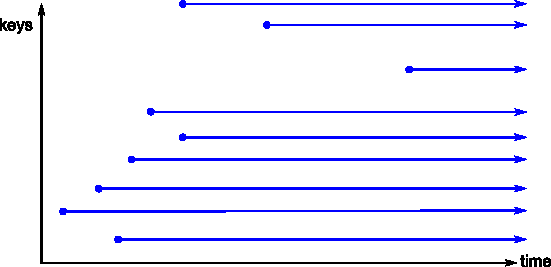
\includegraphics[width=6in]{pqinsert.pdf}}
  \end{center}

  \caption{\small Graph of priority queue featuring only a set of $insert$s}
  \label{fig-pqinsert}
	\rule{\textwidth}{0.005in}
\end{figure}

Every $delete$-$min()$ operation creates a vertical ray that starts at $(t,-\infty)$ and shoots upwards, stopping at the horizontal ray of the element it deletes. Thus, the horizontal ray becomes a line segment with end points $(t,k)$ and $(t_k,k)$, where $t_k$ is the time of key $k$'s deletion.

This combinations of inserts and deletes creates a graph of nonintersecting upside down ``L'' shapes, where each L corresponds to an $insert$ and the $delete$-$min()$ that deletes it.  Elements which are never deleted remain rightward rays. Figure \ref{fig-pqdel} demonstrates this by adding a few $delete$-$min$s to our previous graph of only $insert$s.

\begin{figure}[ht]
	\rule{\textwidth}{0.005in}
  \begin{center}
    \scalebox{.5}{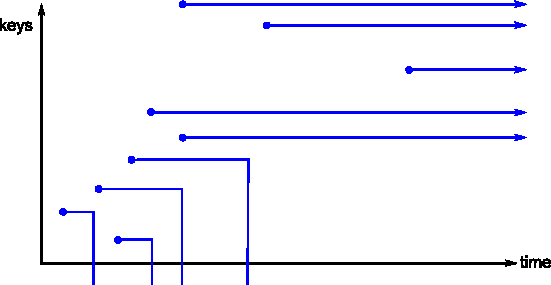
\includegraphics[width=6in]{pqdel}}
  \end{center}

  \caption{\small Adding $del$-$min()$ operations leads to these upside down ``L'' shapes.}
  \label{fig-pqdel}
	\rule{\textwidth}{0.005in}
\end{figure}

The rest of the discussion will focus on $Insert(t,$``$insert(k)$''$)$.  It should be easy enough to convince yourself that $Delete(t,$``$delete$-$min$''$)$ has equivalent analysis if you think about Delete as inserting the deleted element at the time of deletion. 

\begin{figure}[ht]
	\rule{\textwidth}{0.005in}
  \begin{center}
    \scalebox{.5}{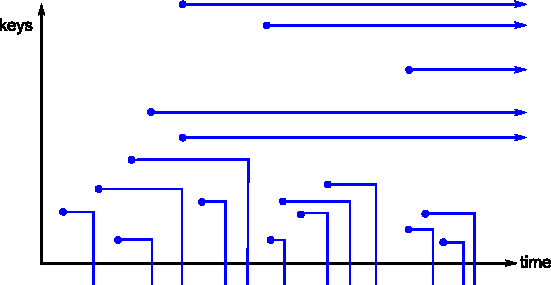
\includegraphics[width=6in]{pqlview}}
  \end{center}

  \caption{\small An L view representation of a priority queue with a more complicated set of updates}
  \label{fig-pqlview}
	\rule{\textwidth}{0.005in}
\end{figure}

Consider the priority queue represented by figure \ref{fig-pqlview}.  It's similar to the previous ones seen but with more inserts and deletes to better illustrate the chain-reactions of retroactive operations.  Figure \ref{fig-pqretro} shows what happens when elements are retroactively inserted.  The retroactive operations and their chain reactions are shown in red.  The cascading changes add up fast.

\begin{figure}[ht]
	\rule{\textwidth}{0.005in}
  \begin{center}
    \scalebox{.5}{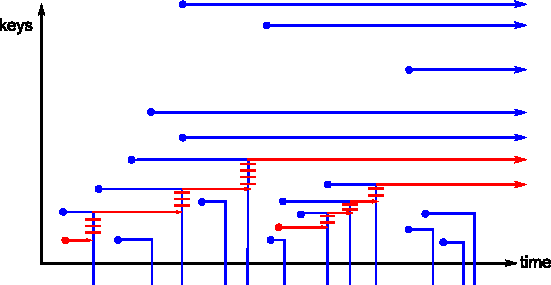
\includegraphics[width=6in]{pqretro}}
  \end{center}

  \caption{\small Retroactive inserts start at red dots and cause subsequent $delete$-$min$ operations to effect different elements as shown.}
  \label{fig-pqretro}
	\rule{\textwidth}{0.005in}
\end{figure}

However, since we're only requiring partial retroactivity we only need to determine what element $Insert(t,$``$insert(k)$''$)$ inserts into $Q_{now}$ where $Q_{now}$ is the priority queue at the present time.  Naively, it is easy to see that the element inserted at $Q_{now}$ is: $\max\left\{k,k' \mid k' \text{ deleted at time} \ge t\right\}$.  That is, the element that makes it to the ``end'' is the biggest element that was previously deleted (ie. the end of the chain-reaction shown in Figure 3) or simply $k$ if it is bigger than those (ie. the insert caused no chain reactions).

\paragraph{Problem:} Maintaining ``deleted'' elements is hard.  It requires us to maintain the various chain-reactions which isn't efficient.  Instead, we would like to simply keep track of inserts.  Such a transformation is possible as long as we define the new concept of ``bridges''.

\begin{definition}
	We define time $t$ to be a bridge if $Q_t \subseteq Q_{now}$.
\end{definition}

This simply means that all of the elements at a bridge $t'$ are also present at $t_{now}$.  You can think of bridges as separating the chaotic chain-reactions that happen during retroactive $Insert$s as seen in figure \ref{fig-pqbridge}.

If $t'$ is the bridge preceding time $t$, then \\ $\max \left\{ k' \mid k' \text{ deleted at time} \ge t \right\} = \max \left\{ k' \notin Q_{now} \mid k' \text{ inserted at time} \ge t' \right\}$


\begin{figure}[ht]
	\rule{\textwidth}{0.005in}
  \begin{center}
    \scalebox{.5}{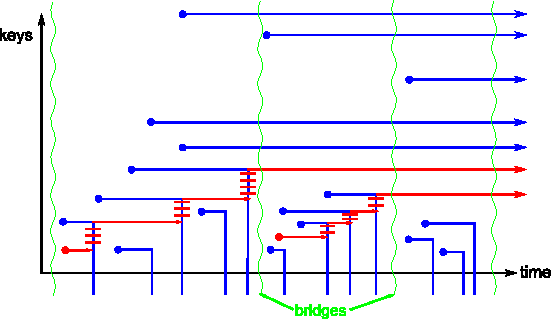
\includegraphics[width=6in]{pqbridge}}
  \end{center}

  \caption{\small Bridges have been inserted as green wavy lines. Notice how they only cross elements present to the end of visible time.}
  \label{fig-pqbridge}
	\rule{\textwidth}{0.005in}
\end{figure}

With that transformation, we only need to maintain three data structures which will allow us to perform partially retroactive operations with only $O(\lg n)$ overhead.

\begin{itemize}
\item We will store $Q_{now}$ as a balanced BST.  It will be changed once per update.
\item We will store a balanced BST where the leaves equal insertions, ordered by time, and augmented with $\forall \text{ node } x: \max\left\{ k' \notin Q_{now} \mid k' \text{ inserted in } x \text{'s subtree} \right\}$.
\item 

\end{itemize}

\subsection{Blah blah blah}
Here is a subsection.

\subsubsection{Blah blah blah}
Here is a subsubsection. You can use these as well.

\subsection{Using Boldface}
Make sure to use lots of boldface.

\paragraph{Question:}
How would you use boldface?

\paragraph{Example:}
This is an example showing how to use boldface to 
help organize your lectures.


\paragraph{Some Formatting.}
Here is some formatting that you can use in your notes:
\begin{itemize}
\item {\em Item One} -- This is the first item.
\item {\em Item Two} -- This is the second item.
\item \dots and here are other items.
\end{itemize}

If you need to number things, you can use this style:
\begin{enumerate}
\item {\em Item One} -- Again, this is the first item.
\item {\em Item Two} -- Again, this is the second item.
\item \dots and here are other items.
\end{enumerate}

\paragraph{Bibliography.}
Please give real bibliographical citations for the papers that we
mention in class. See below for how to include a bibliography section.
If you use BibTeX, integrate the .bbl file into your .tex
source. You should reference papers like this: ``The FKS
dictionary originates in a paper by Fredman, Koml\'{o}s and
Szemer\'{e}di \cite{fks}.'' In general, the name of the authors should
appear in text at most once (for the first citation); further
citations look like: ``Our proof follows that of \cite{fks}''.

Take a look at previous lectures (TeX files are available) to see the
details. A excellent source for bibliographical citations is
DBLP. Just Google DBLP and an author's name.


%\bibliography{mybib}
\bibliographystyle{alpha}

\begin{thebibliography}{77}

\bibitem{fks}
M. Fredman, J. Koml\'{o}s, E. Szemer\'{e}di,
\emph{Storing a Sparse Table with $O(1)$ Worst Case Access Time},
Journal of the ACM, 31(3):538-544, 1984.

\end{thebibliography}

\end{document}
